\documentclass[main.tex]{subfiles}

\begin{document}
	
\section{Постановка задачи}
Поставлена задача условной оптимизации следующего вида:
\begin{gather*}
\overline{\phi_0}(x) \rightarrow min_{x} \\
x \in \overline{\varOmega} := \{x|\phi_1(x) \le 0, \phi_2(x) \le 0\} 
\end{gather*}
где $x \in \mathds{R}^2$, $\phi_1, \phi_2$ -- выпуклые функции, подобранные так, чтобы множество $\overline{\varOmega}$ было замкнутым; $\overline{\phi_0}$ -- нелинейная функция цели.\\
\begin{enumerate}
	\item Привести задачу к виду, пригодному для применения метода отсекающей гиперплоскости:
	\begin{gather*}
	\phi_0(x) = (c, x) \rightarrow min_{x} \\
	x \in \varOmega := \{x|\phi(x) \le 0\} 
	\end{gather*}
	где $\phi$ -- выпуклая функция.
	\item Построить замкнутый многогранник $S:=\{x|Ax\le b\}$ с условием $\varOmega \subset S$, необходимый для начального этапа метода отсекающей гиперплоскости.
	\item Решить задачу методом отсекающей гиперплоскости, на каждом шаге решая проблему линейной минимизации следующим образом: проблему привести к двойственному виду, применить симплекс-метод и восстановить решение прямой по решению двойственной.
\end{enumerate}

\section{Обоснование применимости методов}
\subsection{Совпадение субградиента с градиентом}
Вспомним теорему из прошлого семестра.\\
Теорема:\\
Пусть $S$ непустое выпуклое множество (в нашем случае параллелепипед).\\
Пусть $\phi(x)$ выпуклая и дифференцируемая.\\
Тогда для любой внутренней точки субградиент совпадает с градиентом функции.
\subsection{Сведение к линейной задаче}
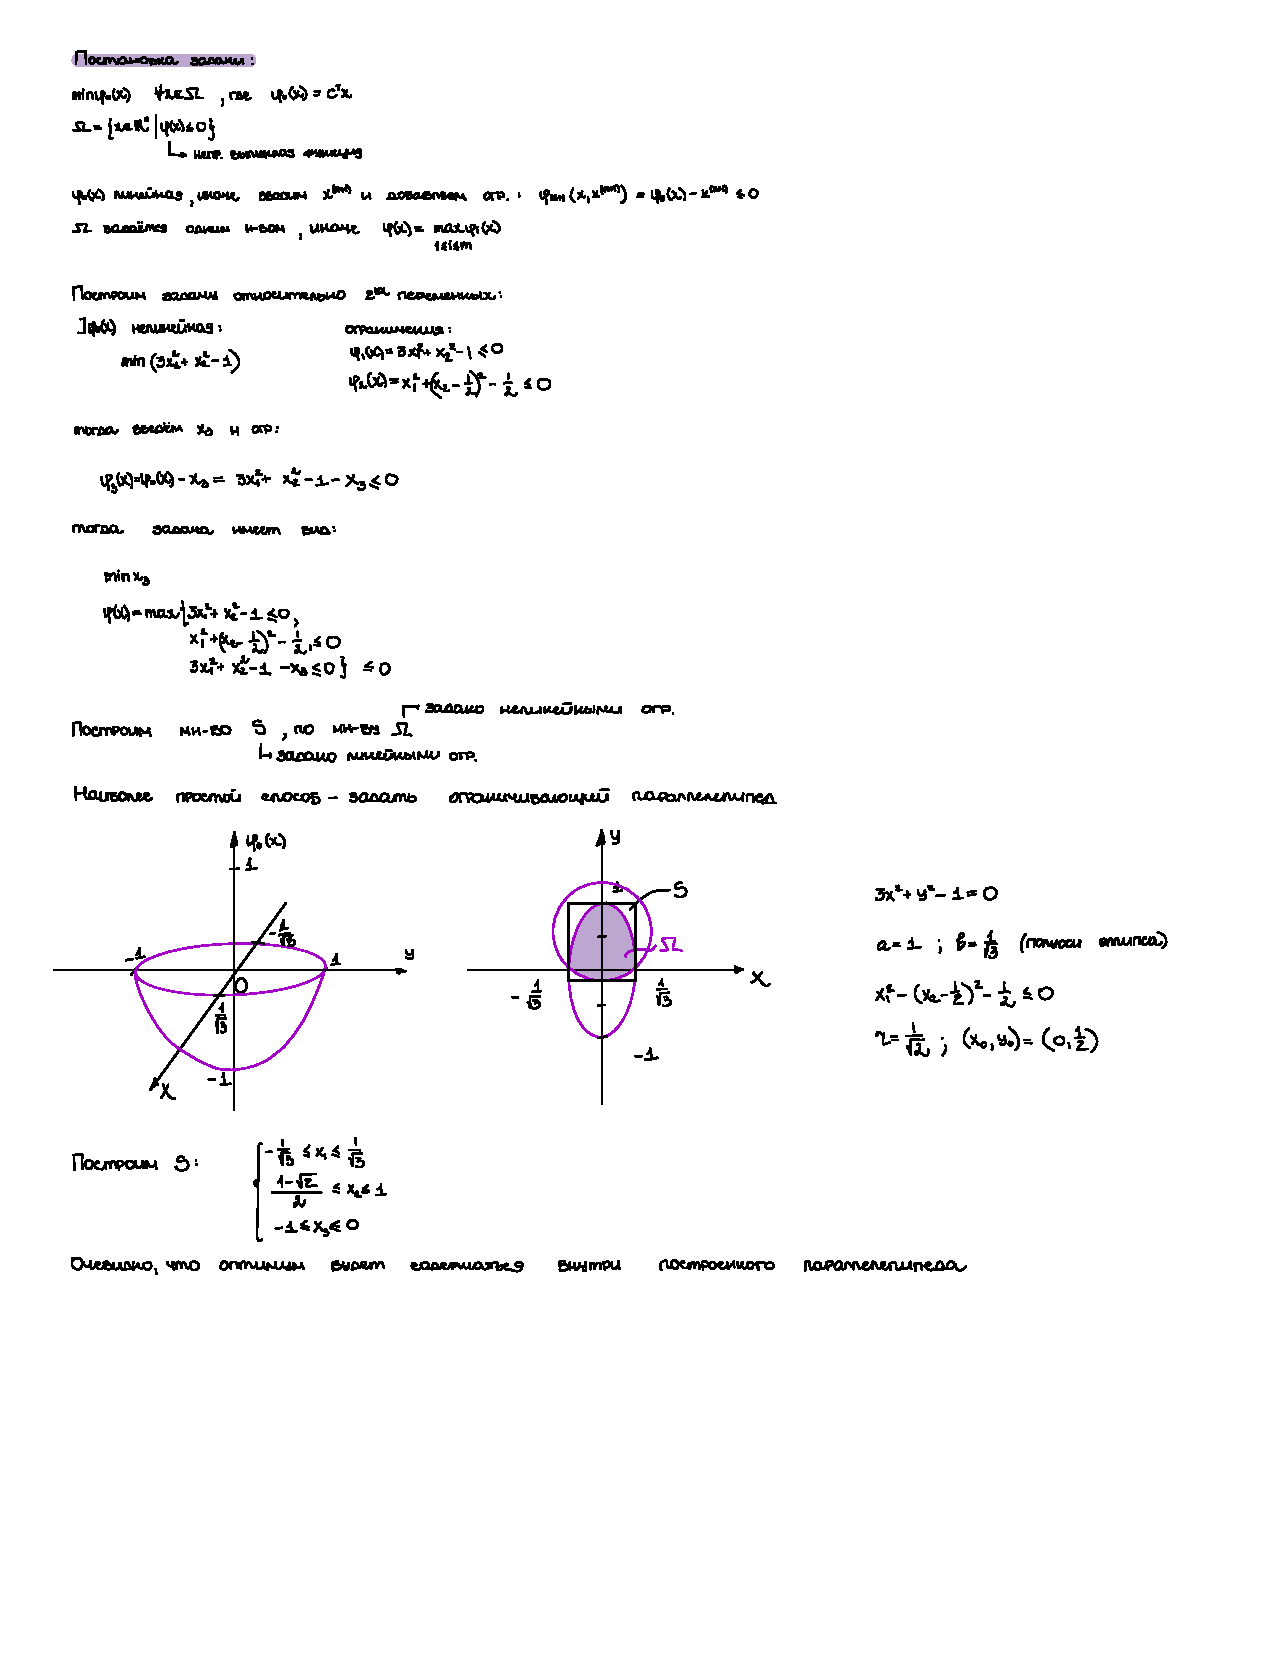
\includepdf[pages=-]{мо.pdf}

\newpage
\section{Описание алгоритмов}
\subsection{Схема алгоритма отсекающей гиперплоскости}
Будем считать, что мы построили выпуклый многогранник $S$, $\varOmega \subset S$; также будем считать, что нам известна функция $\phi$, определяющая множество $\varOmega$, и в каждой точке мы можем вычислить её субградиент $\underline{\nabla}\phi(x)$. Зададим параметр окончания вычислений $\varepsilon$: если на какой-то итерации мы не сместились  по сравнению с предыдущей точкой больше, чем на $\varepsilon$ по норме, выйдем из процесса итераций.\\
Тогда применяется следующий алгоритм \cite{boldirev}:
\begin{enumerate}
	\item К задаче $(x,c) \rightarrow min_x, x \in S:={x|A\cdot x\le b}$ составляется двойственная: 
	$$(y,-b) \rightarrow min_y, y \in \overline{S}:={|A^T\cdot y = c, y \ge 0}$$
	Эта задача решается методом перебора опорных векторов \cite{petuh}. Результат (минимизирующий целевую функцию вектор $y^*_0$, опорный к $S$, и его базис $N_k \in N$, где $N$ - множество индексов строк матрицы $\overline{A}$, $\overline{A} = A^T$) запоминаются. 
	\item По найденным $N_k$ и $A$ восстанавливается решение прямой задачи (алгоритм описан в \ref{section:restore}).
	\item Далее в цикле проверяется условие $x^* \in \varOmega$. Если условие выполнено, $x^*$ -- решение, цикл завершается. Иначе проводится процедура \emph{cutting\_plane\_iteration}, описанная ниже. Эта процедура выдаёт следующий многогранник $S^{'}$ и решение прямой и двойственной задачи на нём - $x^{*'}, y^{*'}, N_k^{'}$. После этого проверяется условие $\norm{x^*-x^{*'}} \le \varepsilon$. Если условие выполнено, прекращаем итерационный процесс; в противном случае полагаем $x=x^{*'}$, $y=y^{*'}$, $N_k=N_k^{'}$ и продолжаем цикл.
\end{enumerate}

\begin{algorithm}[H]
	\KwData{$ \varepsilon > 0$;\newline
		 $x^*$, $y^*$, $N_k$ -- результат решения обратной и прямой задачи; \newline
		 $A, b, c$ -- параметры прямой задачи; \newline
	     $\phi(x), \underline{\varDelta}\phi(x)$ - информация о целевой функции}	
	\KwResult{
		$A^{'}, b^{'}, c^{'}$ -- новые параметры прямой задачи линейного программирования \newline
		$x^{*'}, y^{*'}, N_k^{'}$ -- решение новой задачи}
	 
	$a_1 := - \underline{\nabla} \phi(x^*)$ - вектор\;
	$b_1 :=  - \phi(x_k)+ (a_1, x_k)$ \;
	$A^{'} := \begin{pmatrix}A\\a_1\end{pmatrix}$ \;
	$b^{'} := \begin{pmatrix}b\\b_1\end{pmatrix}$\;
	Записать двойственную задачу к задаче с параметрами $A^{'}, b^{'}, c^{'}$\;
	Решить двойственную задачу симплекс-методом, в качестве начального приближения взяв вектор $y^{'}$\;
	Восстановить решение прямой задачи, пользуясь методом, описанном в секции \ref{section:restore}.
	
	\caption{Процедура \emph{cutting\_plane\_iteration}}
\end{algorithm}

\subsection{Алгоритм вычисления субградиента}
\begin{enumerate}
	\item Найдем множество индексов $I(x_k) = \{i | \phi_i(x_k)=\max(\phi_i(x_k), 1 \leq i \leq m)\} $, $m$ - размерность задачи (в нашем случае $m = 3$).
	\item Вычислим  $\nabla\phi_i(x_k)$ для любого индекса из множества $I(x_k)$ 
\end{enumerate}

 
\subsection{Восстановление результатов прямой задачи} \label{section:restore}
Пусть прямая задача линейного программирования дана в форме
\begin{gather*}
\phi_0(x) = (c, x) \rightarrow min_{x} \\
x \in S := \{x|Ax \le b\} 
\end{gather*}
Тогда двойственная форма такова:
\begin{gather*}
(c_1, y) \rightarrow min_{y} \\
y \in S_1 := \{x|A_1 = b_1, x \ge 0\}\\
c_1 = -b\\
b_1 = c\\
A_1 = A^T\\
\end{gather*}
Если матрица $A_1=A_1[M,N]$ (соответственно, $b_1 = b_1[M]$, $c_1 = c_1[N]$) и $y^*$ - решение двойственной задачи, т. е. некий опорный вектор с базисом $A[M, N_k], N_k \in N$, то несложно восстановить решение прямой задачи:\\
$$ x^* = c \cdot (A[M, N_k])^{-1}$$
\section{Результаты решения задачи}
При запуске алгоритма с построенным множеством $S$ на четвёртой итерации была найдена точка, удовлетворяющая условию выхода по малости нормы разности с предыдущим опорным вектором: в трёхмерном пространстве это $x^* = \begin{pmatrix}0\\0.5 \\ 0\end{pmatrix}$ (соответственно, при переходе обратно на плоскость -- $\begin{pmatrix}0\\0.5 \end{pmatrix}$). \\
\section{Оценка достоверности полученных результатов}
Проверим: $\phi(0, 0.5, 0) = max(-0.75, -0.5, -0.75) = -0.5$\\ \\
После приведения выбранной задачи к виду, пригодному для применения метода, она будет иметь такой вид: 
$$min\{\phi_0(x)\} = min\{x_3\}, x \in \Omega$$
$$\Omega = \{x \in \mathds{R}^3 | \phi(x) \leq 0\}$$
$$\phi(x) = max\{3x_1^2 + x_2^2 - 1, x_1^2 + (x_2 -\frac{1}{2})^2 - \frac{1}{2}, 3x_1^2 + x_2^2 - 1 - x_3\}, x \in \mathds{R}^3$$
\begin{equation*}
S = S_0 = 
\begin{cases}
-\frac{1}{\sqrt(3)} \leq x_1 \leq \frac{1}{\sqrt(3)}\\
\frac{1-\sqrt(2)}{2} \leq x_2 \leq 1\\
-1 \leq x_3 \leq 0
\end{cases}
\end{equation*}
Проверим условия теоремы о сходимости алгоритма \cite{petuh}:
\begin{enumerate}
	\item $\phi(x)$ - непрерывная выпуклая функция:\\
	Непрерывность $\phi$ очевидна.
	Выпуклость следует из того, что каждая из трёх функций, максимумом из которых является $\phi$ выпукла, а максимум из выпуклых функций -- выпуклая функция.
	\item $\Omega$ - компактная область:\\
	Ранее был построен параллелепипед $S$, в который мы погрузили область $\Omega \Longrightarrow$ огранниченность точно есть.
	Из того, что все неравенства в определении $\phi$ строгие и функция $\phi$ кусочно-непрерывно дифференцируемая в области $S$, следует замкнутость $\varOmega$ как срезки надграфика $\phi$.\\
	Замкнутые ограниченные множества в $\mathds{R}^n$ компактны.
	\item $\forall x \in S_0 \hookrightarrow \|a(x)\| \leq R$ - субградиент $\phi(x)$ в каждой точке $S_0$ ограничен:\\
	Согласно алгоритму вычисления субградиента в точке, описанному выше, можем заметить, что, какой бы индекс из $I(x)$ мы ни взяли для вычисления $a(x) = \nabla \phi_i(x)$, норма $\|a(x)\|$ всегда останется ограниченной внутри параллелепипеда:
	\begin{itemize}
		\item Если $a(x) = \nabla\phi_1(x) = (6x_1, 2x_2, 0)$, то $\|a(x)\|$ очевидно ограничена внутри $S_0$.
		\item Если $a(x) = \nabla\phi_2(x) = (2x_1, 2x_2 - 1, 0)$, то $\|a(x)\|$ тоже очевидно ограничена внутри $S_0$.
		\item Если $a(x) = \nabla\phi_3(x) = (6x_1, 2x_2, -1)$, то $\|a(x)\|$ тоже очевидно ограничена внутри $S_0$.
	\end{itemize}
	Возьмем за R максимальную из констант, ограничивающих $\|\nabla\phi_i\|$ на $S$.
\end{enumerate}
Таким образом, можем быть уверены, что метод применим к данной задаче и любая предельная точка последовательности приближений, которую мы строим, является оптимальной.


\end{document}